\section{User Study Evaluation}

We conducted our study as outlined in the Implementation section, aiming to investigate the following hypotheses:

\begin{itemize}[itemsep=-0.3em]
    \item \textbf{H1}: Is there a difference in task performance when interacting with the volumetric display in 3D as opposed to 2D?
    \item \textbf{H2}: Is there a difference in task performance when interacting with the volumetric display directly with hands as opposed to via teleoperation?
\end{itemize}

\subsection{Participants}
The study took place between the 1st and 5th of June in Room 218 of the Huxley Building at Imperial College London's South Kensington Campus. We were able to engage 16 participants in our study, 14 of whom consented to be photographed, as shown in Fig~\ref{fig:users}.

\begin{figureBox}[label={fig:users}, width=1.0\linewidth]{Participants}
    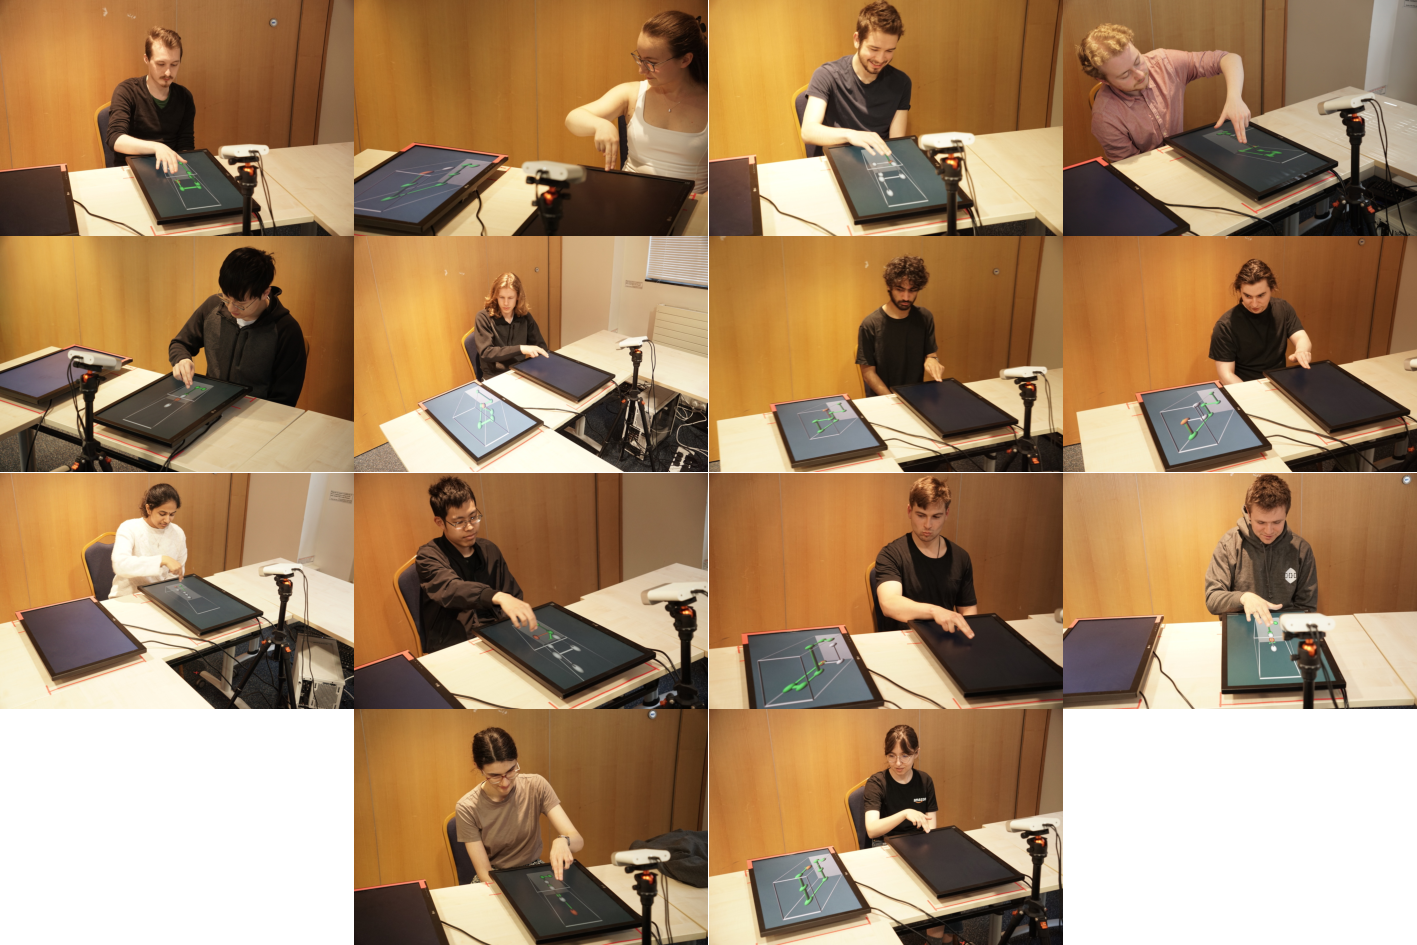
\includegraphics[width = 1.0\linewidth]{./evaluation/figures/users.pdf}
\end{figureBox}

The recruitment of participants was primarily facilitated through existing networks, involving colleagues and acquaintances. Attempts to recruit participants through other channels proved less effective. \\

Consequently, our participant sample was not broadly representative of the wider population. The majority of participants were concentrated around the age of 22, as depicted in Fig~\ref{fig:participant-age}, and the group was predominantly male, as illustrated in Fig~\ref{fig:participant-gender}. \\

We also surveyed our participants regarding factors we anticipated might influence the study. Notably, 37\% of the participants wore glasses during the study (Fig~\ref{fig:participant-glasses}), and almost every participant had prior experience with VR (Virtual Reality) or AR (Augmented Reality), as shown in Fig~\ref{fig:participant-vr-us}. Our analysis indicated that these variables did not significantly impact the study results.

\begin{invisBox}
	\pictureBox[label={fig:participant-age}]{Age}{
	  \adjustbox{height=6cm, keepaspectratio}{
		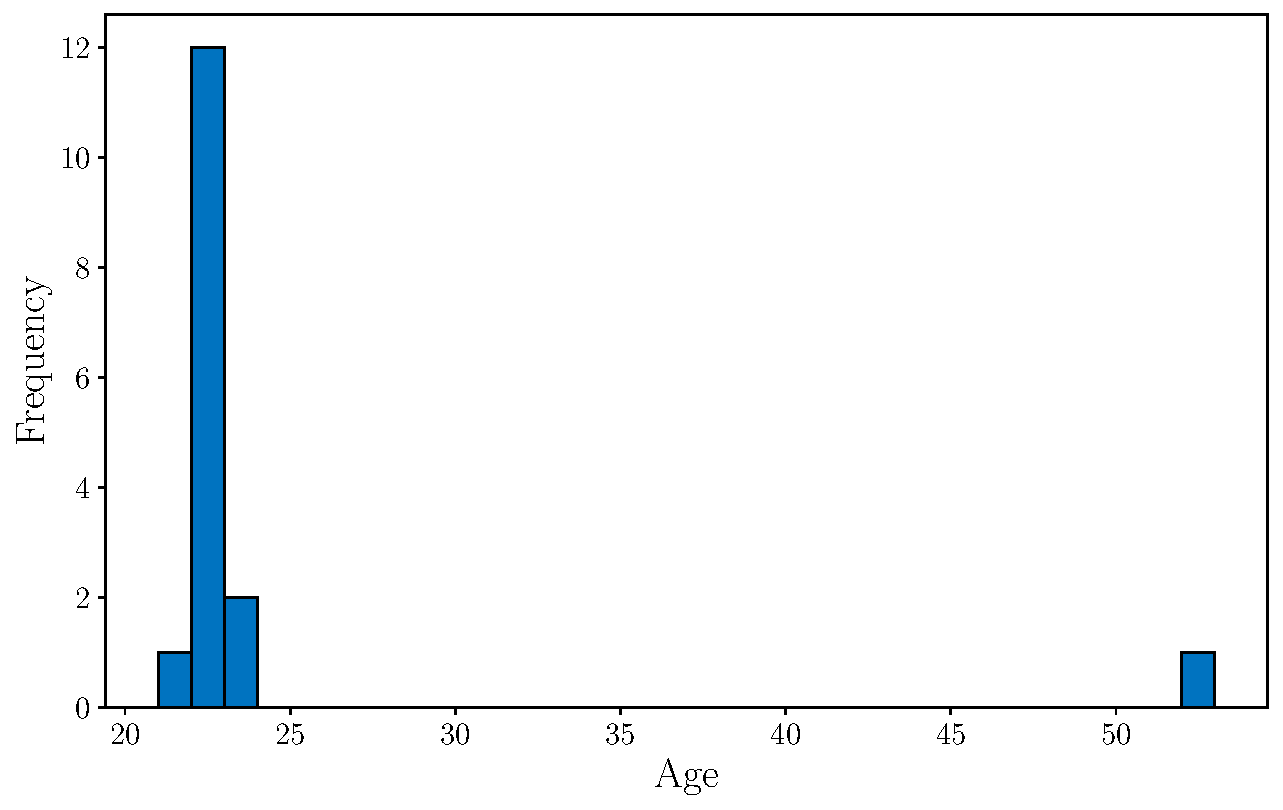
\includegraphics{./evaluation/figures/survery/age-distribution.pdf}
	  }
	}
	\hfill
	\pictureBox[label={fig:participant-glasses}]{Glasses}{
	\adjustbox{height=6cm, keepaspectratio}{
	  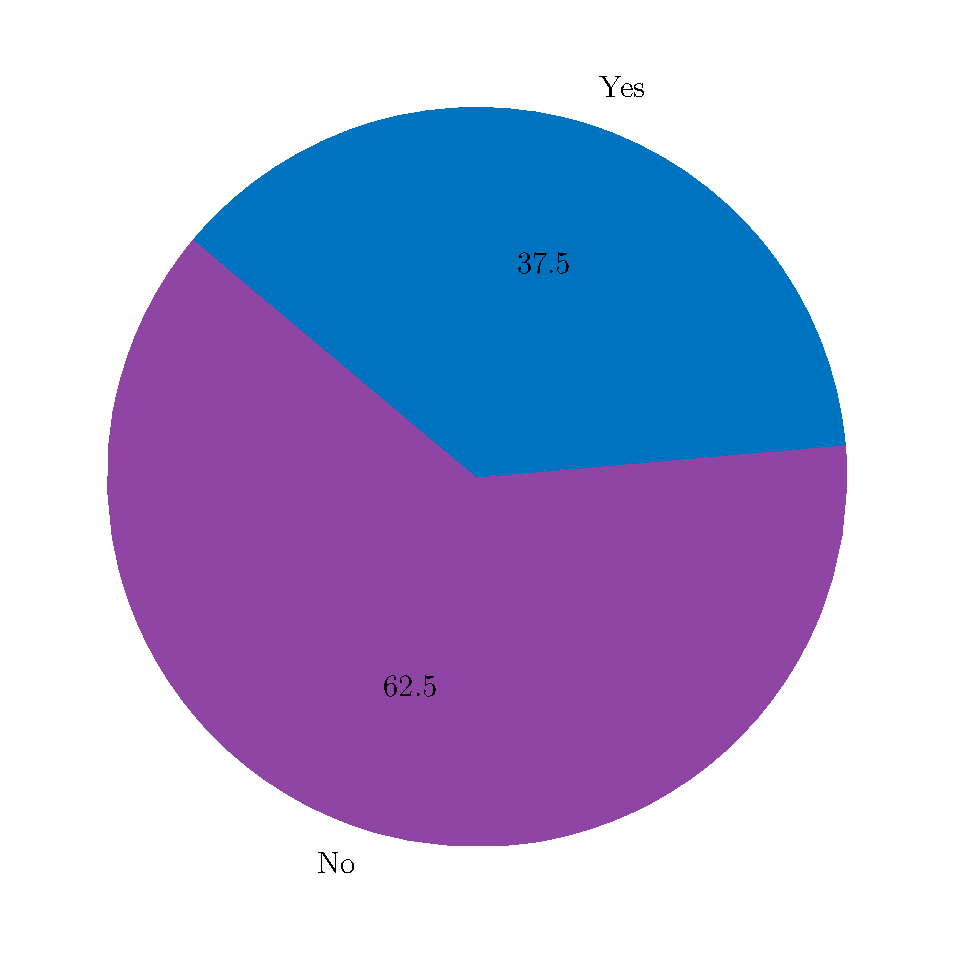
\includegraphics{./evaluation/figures/survery/glasses-distribution.pdf}
	  }
	}
	\\[0.3cm]
	\pictureBox[label={fig:participant-vr-us}]{Used VR/AR}{
	  \adjustbox{height=7.75cm, keepaspectratio}{
		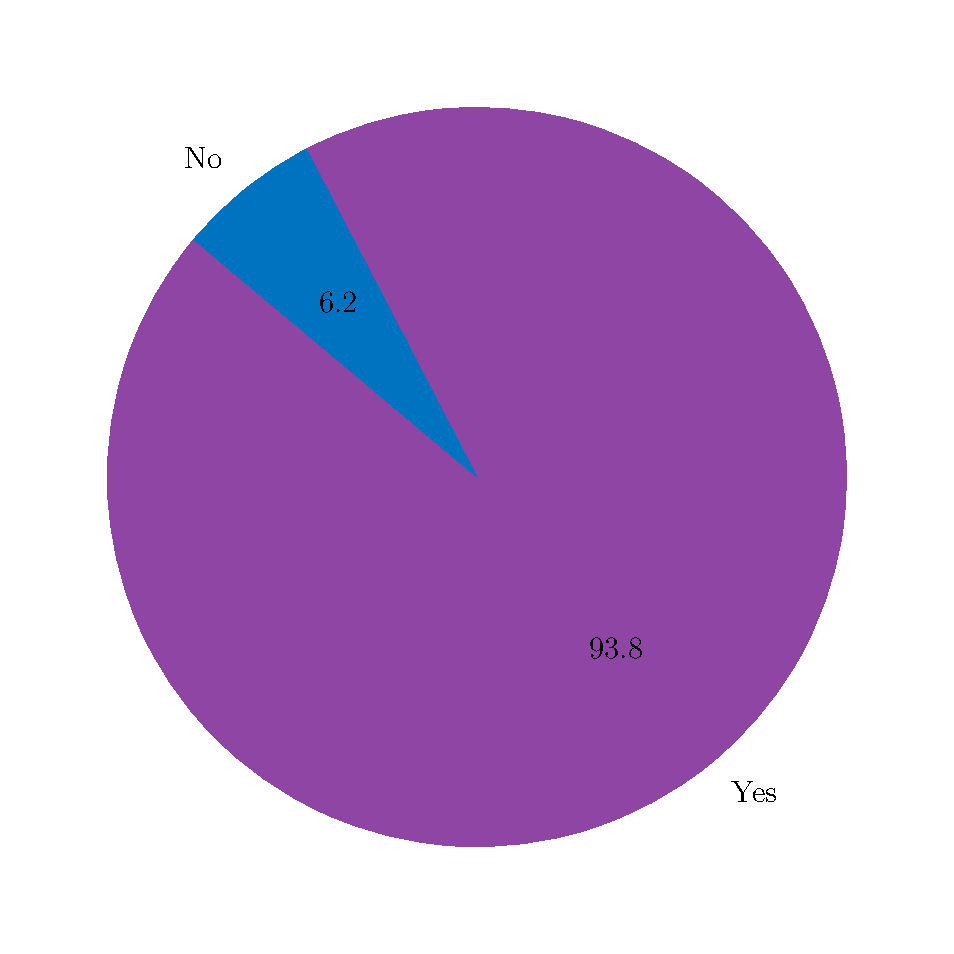
\includegraphics{./evaluation/figures/survery/vr-ar-distribution.pdf}
	  }
	}
	\hfill
	\pictureBox[label={fig:participant-gender}]{Gender}{
	\adjustbox{height=7.75cm, keepaspectratio}{
	  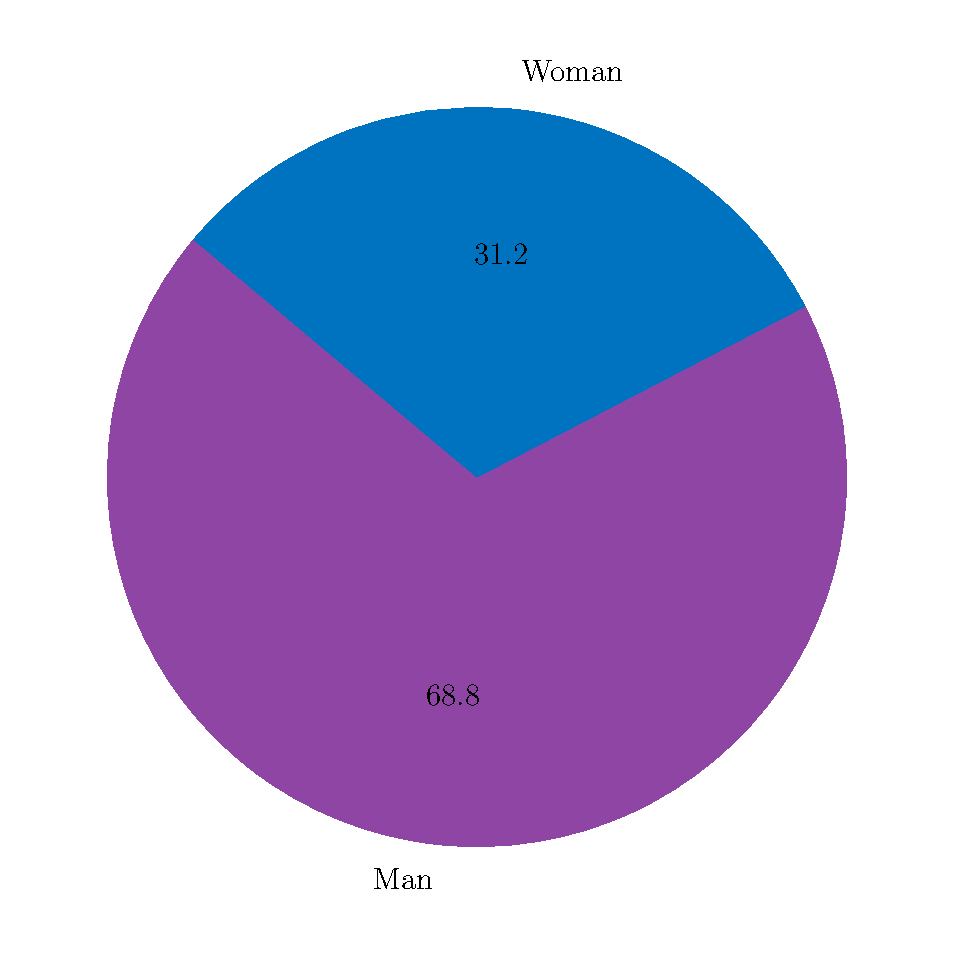
\includegraphics{./evaluation/figures/survery/gender-distribution.pdf}
	  }
	}
\end{invisBox}

\subsubsection{Results: Timings}
Upon completing the study with all participants, we collected and analyzed the data, focusing particularly on the time taken to complete each segment of the tasks. Our analysis revealed that both the type of view (STATIC, i.e., 2D, versus TRACKER, i.e., 3D) and the presence of an offset (OFFSET versus NO OFFSET) had a statistically significant impact on the time required to complete the segments. We plotted the average segment completion time against these variables in Fig~\ref{fig:anova-interaction}.

\begin{figureBox}[label={fig:anova-interaction}, width=0.8\linewidth]{Interaction between View and Offset on Segment Completion Times}
    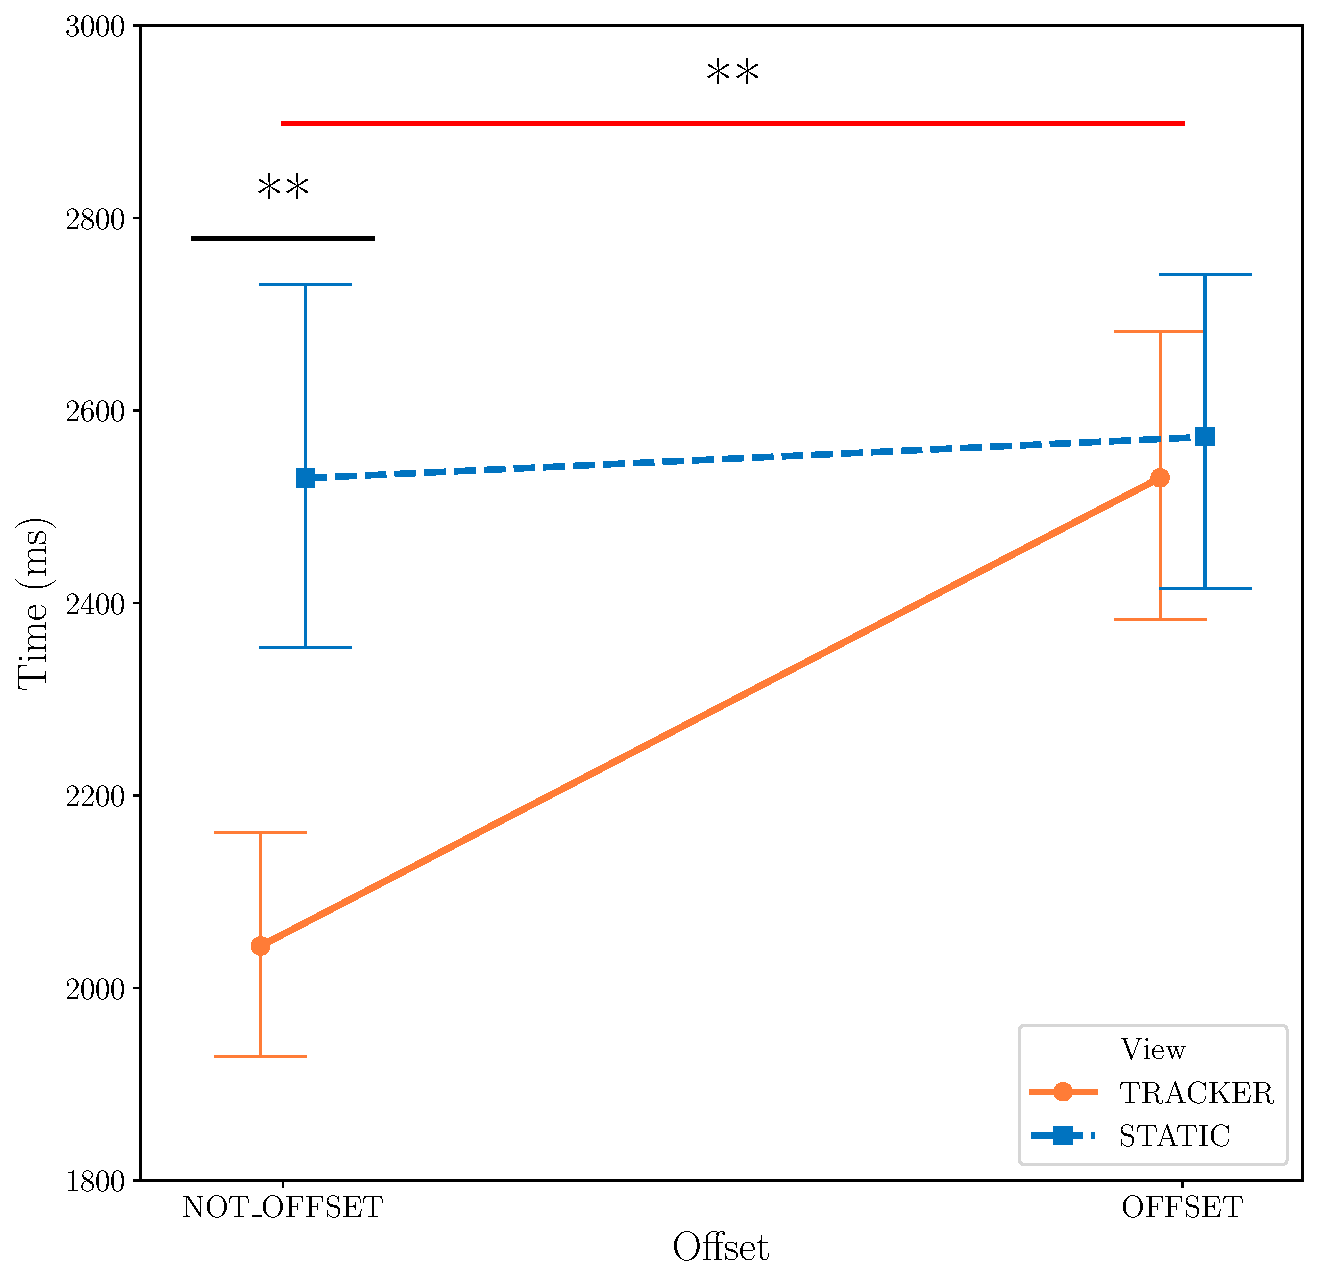
\includegraphics[width = 1.0\linewidth]{./evaluation/figures/survery/anova-interaction.pdf}
\end{figureBox}

To confirm the significance of these results, we conducted a type II ANOVA test, the results of which are displayed in Table~\ref{tab:anova}. \\

\begin{table}[h!]
	\stepcounter{globalFigureCounter}
	\centering
	\caption{ANOVA Results for Fig~\ref{fig:anova-interaction}}
	\label{tab:anova}
	\begin{tabular}{lS[table-format=1.2e+2]S[table-format=4.0]S[table-format=2.6]S[table-format=1.6]}
		\toprule
		\textbf{Source} & \textbf{Sum of Squares} & \textbf{df} & \textbf{F} & \textbf{p-value} \\
		\midrule
		\texttt{C(View)} & 3.363186e+07 & 1.0 & 10.698212 & 0.001092 \\
		\texttt{C(Offset)} & 3.341680e+07 & 1.0 & 10.629800 & 0.001132 \\
		\texttt{C(View):C(Offset)} & 2.344484e+07 & 1.0 & 7.457744 & 0.006375 \\
		\texttt{Residual} & 5.985586e+09 & 1904.0 & NaN & NaN \\
		\bottomrule
	\end{tabular}
\end{table}

The data suggests that participants performed best when using the TRACKER mode (3D view) directly in front of them, completing segments in an average of 2043 ms. Performance deteriorated under other conditions, with average completion times of 2530 ms for STATIC, 2573 ms for STATIC OFFSET, and 2530 ms for TRACKER OFFSET, respectively. This indicates that the advantage of the 3D view is significant only when the display is directly in front of the user, and this benefit diminishes when an offset is introduced. \\

We hypothesize that this phenomenon is due to motion parallax, an effect where closer objects appear to move more relative to farther objects. This effect is crucial for depth perception in the real world and contributes to the effectiveness of 3D displays. However, when the 3D display is offset, the motion parallax effect is reduced, diminishing the advantages of the 3D display. \\

Interestingly, the data suggests that the offset condition does not significantly impact the time taken to complete the segments, contrary to our expectations. We hypothesized that the offset would significantly affect task completion time, potentially because the user's hand might occlude their view when the display is directly in front. This hypothesis is supported by our observation that participants moved their heads equally, regardless of the offset condition, as shown in Fig~\ref{fig:eye-movement}. This suggests that participants were still attempting to obtain a better view of the segments even when they were offset. \\

To further investigate this phenomenon, it would be prudent to conduct additional studies examining multiple offset conditions with varying distances. This approach would enable us to measure more precisely the decline in the effectiveness of the TRACKER mode as the offset distance increases, providing further validation of our motion parallax hypothesis. It would also be insightful to try 
offsetting the interaction zone rather the display to check if this has an effect.

\begin{figureBox}[label={fig:eye-movement}, width=0.8\linewidth]{Combined Mean Eye Movement Values Per Millisecond and Standard Deviations}
    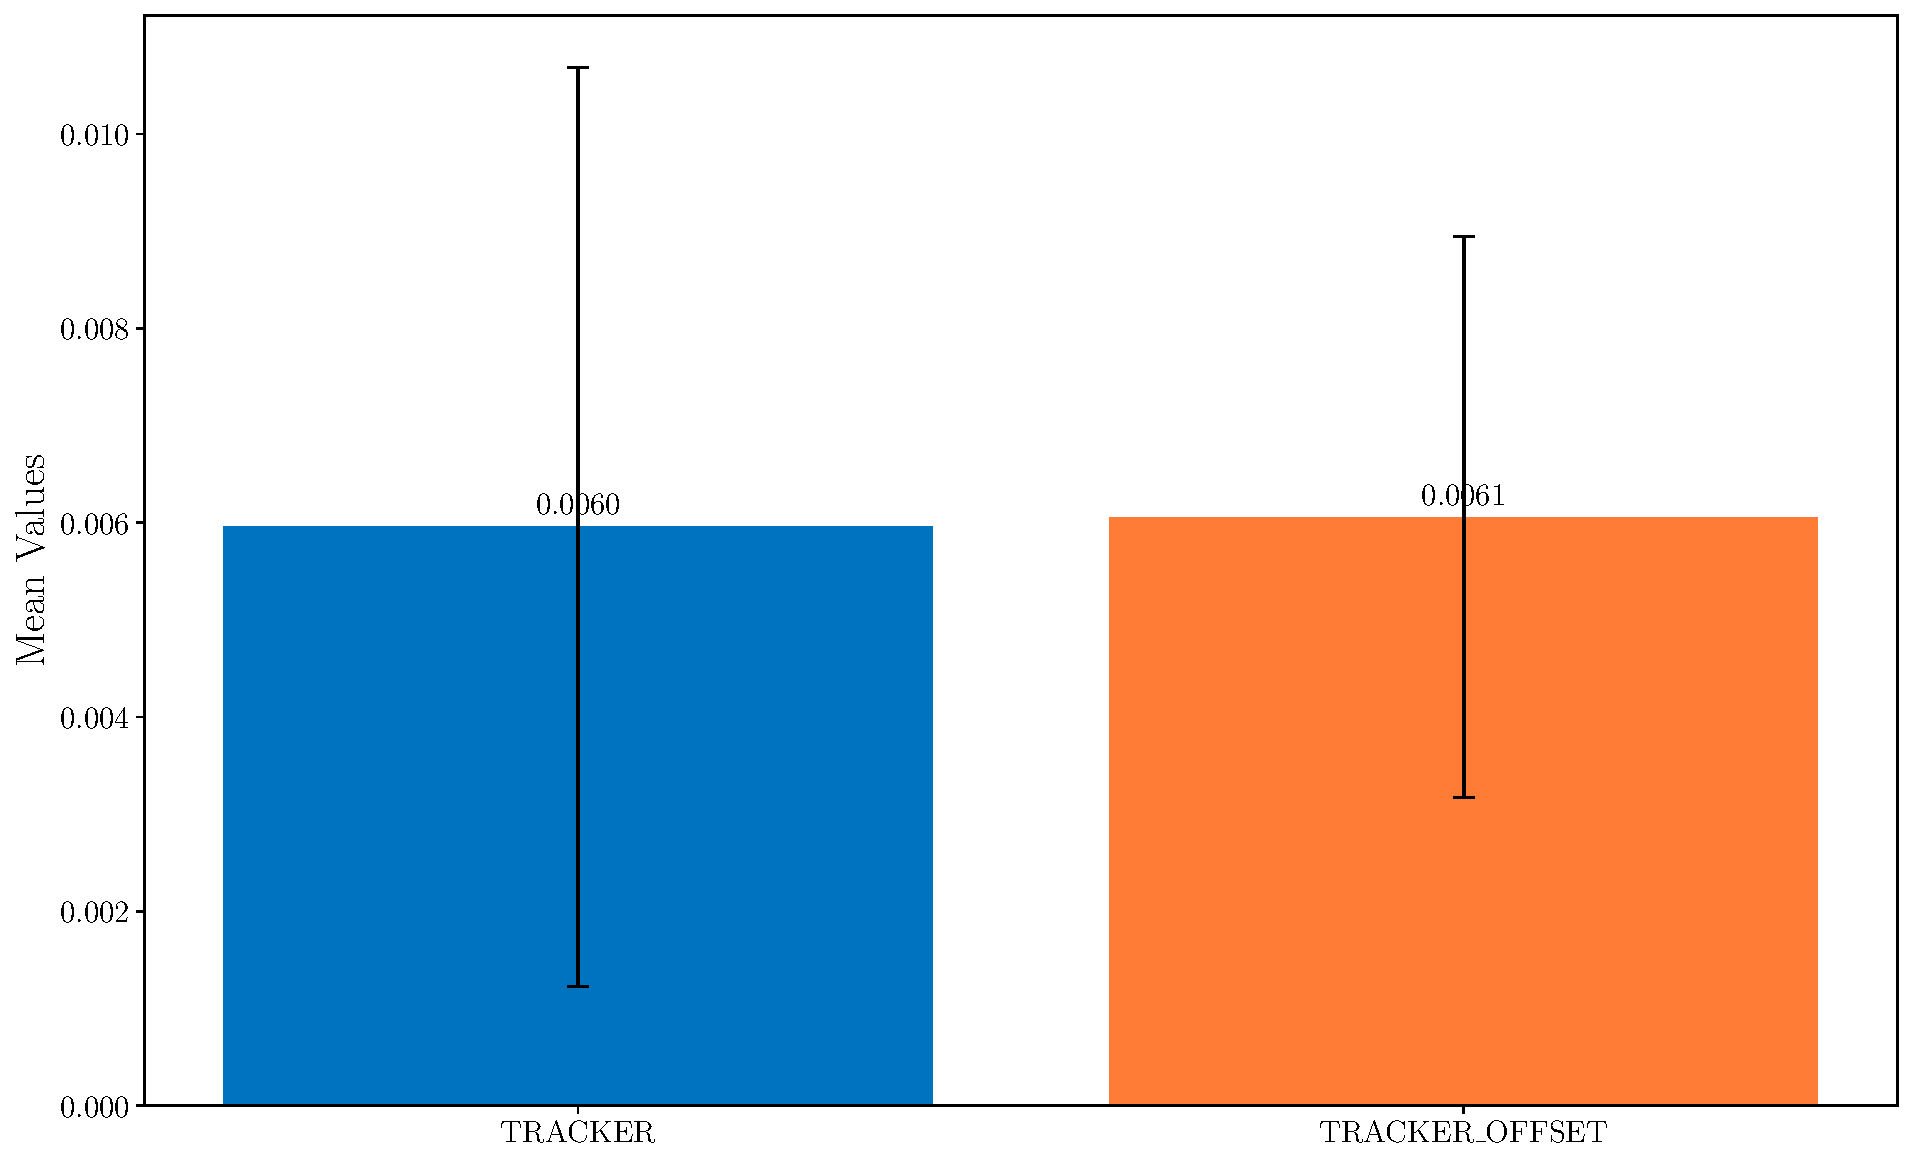
\includegraphics[width = 1.0\linewidth]{./evaluation/figures/survery/combined-eye-movement.pdf}
\end{figureBox}

As demonstrated in Table~\ref{tab:ttest}, the t-test results indicate that the offset condition does not have a significant effect on eye or head movement.

\begin{table}[h!]
	\stepcounter{globalFigureCounter}
    \centering
    \caption{T-Test Results for Fig~\ref{fig:eye-movement}}
    \label{tab:ttest}
    \begin{tabular}{lS[table-format=2.4]S[table-format=1.6]}
        \toprule
        \textbf{Statistic} & \textbf{Value} & \textbf{p-value} \\
        \midrule
        \texttt{T-statistic} & -0.4170 & 0.6767 \\
        \bottomrule
    \end{tabular}
\end{table}

\subsubsection{Results: Hand Precision}

Another important metric we investigated was the distance of the user's hand from the end of the segment they were attempting to select over time. This distance represents their error over time, with a value of 0 indicating that the user successfully overlapped their finger with the target, thereby completing the task. The distribution of these distances is illustrated in Fig~\ref{fig:distance-distribution}. \\

We observed that in both the STATIC OFFSET and TRACKER OFFSET conditions, users exhibited significantly worse precision in selecting the point at the end of the segment. These conditions showed a much larger peak just before reaching a distance of zero, which is the target point that participants were trying to precisely select. Interestingly, the STATIC condition had a much smaller peak near completion, closely resembling the TRACKER condition, but was consistently worse than every other condition throughout the task. \\

\begin{figureBox}[label={fig:distance-distribution}, width=1.0\linewidth]{Distribution of Hand Distances from Segment End}
    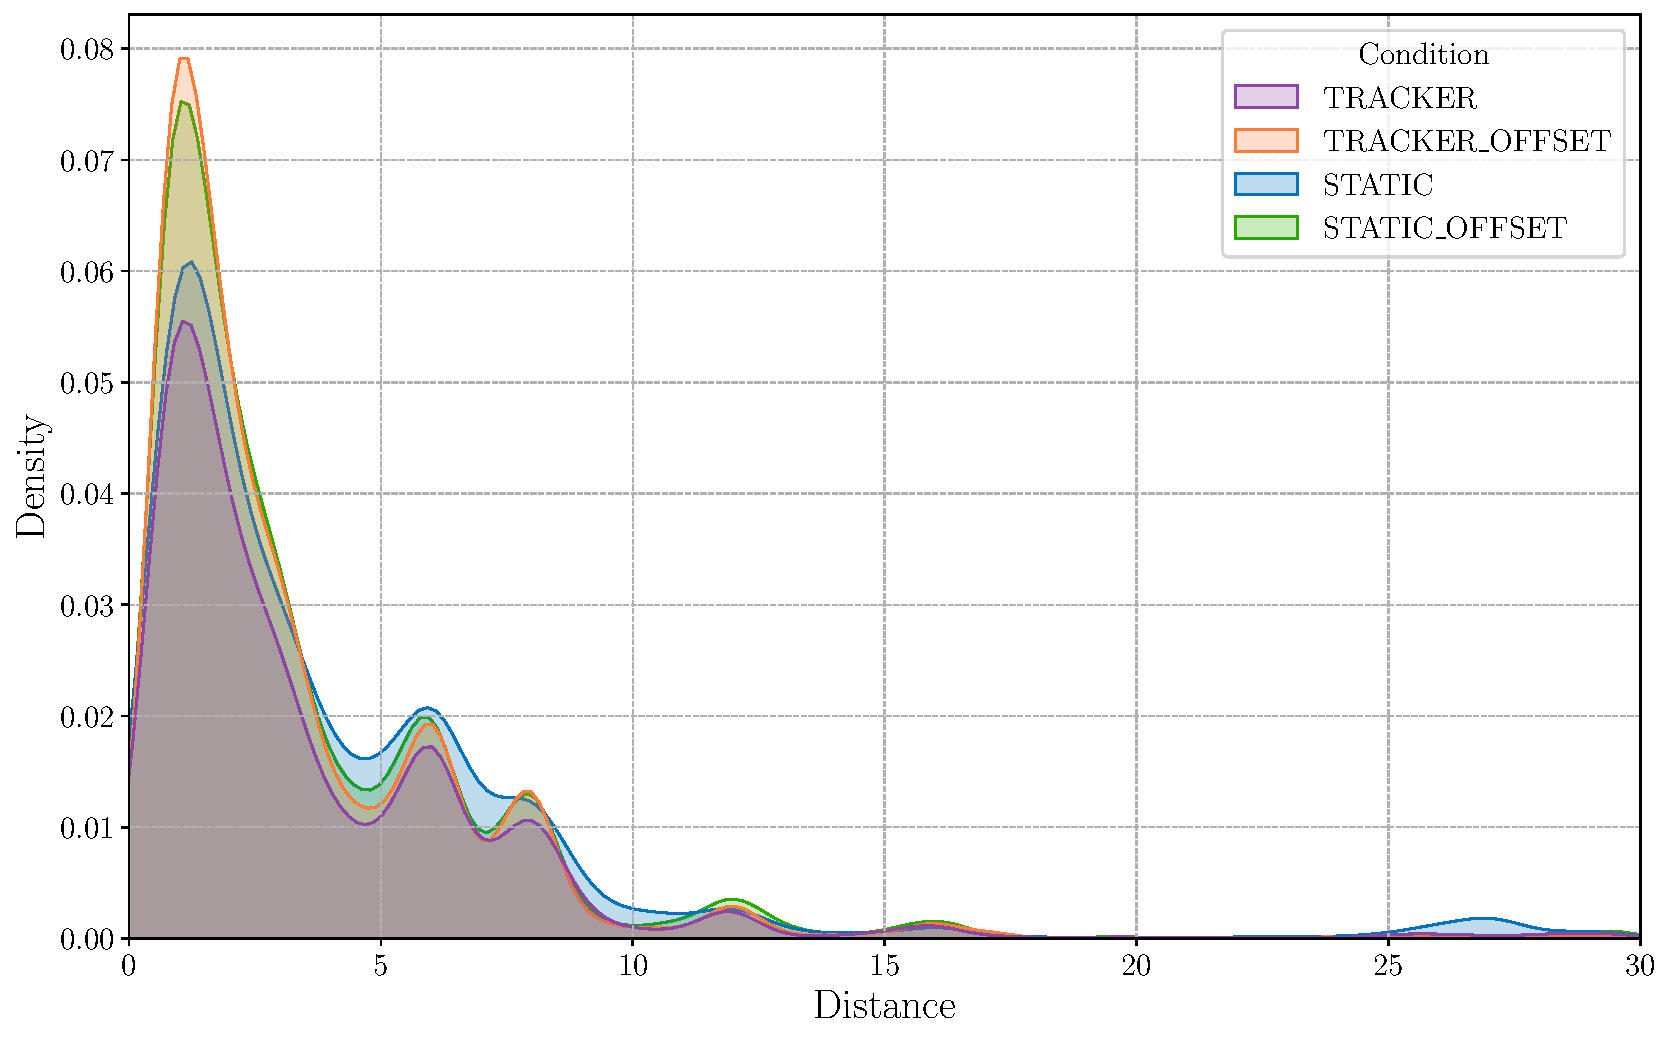
\includegraphics[width = 1.0\linewidth]{./evaluation/figures/survery/distance-distribution.pdf}
\end{figureBox}

We hypothesize that the significantly worse performance in the OFFSET conditions is due to the lack of motion parallax, which would make it more challenging for users to judge the precise distance and depth between their hand and the end of the segment. This difficulty likely resulted in users spending more time at the end of a segment trying to precisely select the final point. Additionally, the display being further away may have made the task appear smaller and more difficult to gauge accurately. \\

In the STATIC condition, users seemed to struggle more consistently with distance throughout the entire task. This difficulty is suggested by the small pronounced peak between 25-30 cm, which we hypothesize was called by users moving their hand in completely incorrect directions. We believe this may be due to the perspective in the STATIC condition being more challenging than in the STATIC OFFSET condition, as users were positioned above and behind the display rather than above, behind, and to the side. Each segment being oriented along the x, y, or z axis may have led to more overlapping segments in the STATIC condition, complicating the user's ability to discern the correct direction. Although this issue was also presumably present in the TRACKER conditions, users could mitigate it by changing their perspective. \\

It is noteworthy that the observed peaks in the distance distributions are likely due to the time it takes for users to realize they have completed a segment and need to start moving towards the next point. We are confident in this interpretation, as the peaks align closely with the lengths of the segments (e.g., 2 cm for one segment, 3 cm for eight segments, 6 cm for twelve segments, 8 cm for ten segments, 12 cm for three segments, and 16 cm for one segment).

\subsection{Survey Results}

Another source of our evaluation was a survey conducted after the study. The survey aimed to gather feedback on the users' experiences and preferences regarding the different conditions they encountered. Participants were asked to rank the conditions in order of preference, as shown in Fig~\ref{fig:condition-preferences}. \\

\begin{figureBox}[label={fig:condition-preferences}, width=1.0\linewidth]{Study Condition Rankings}
    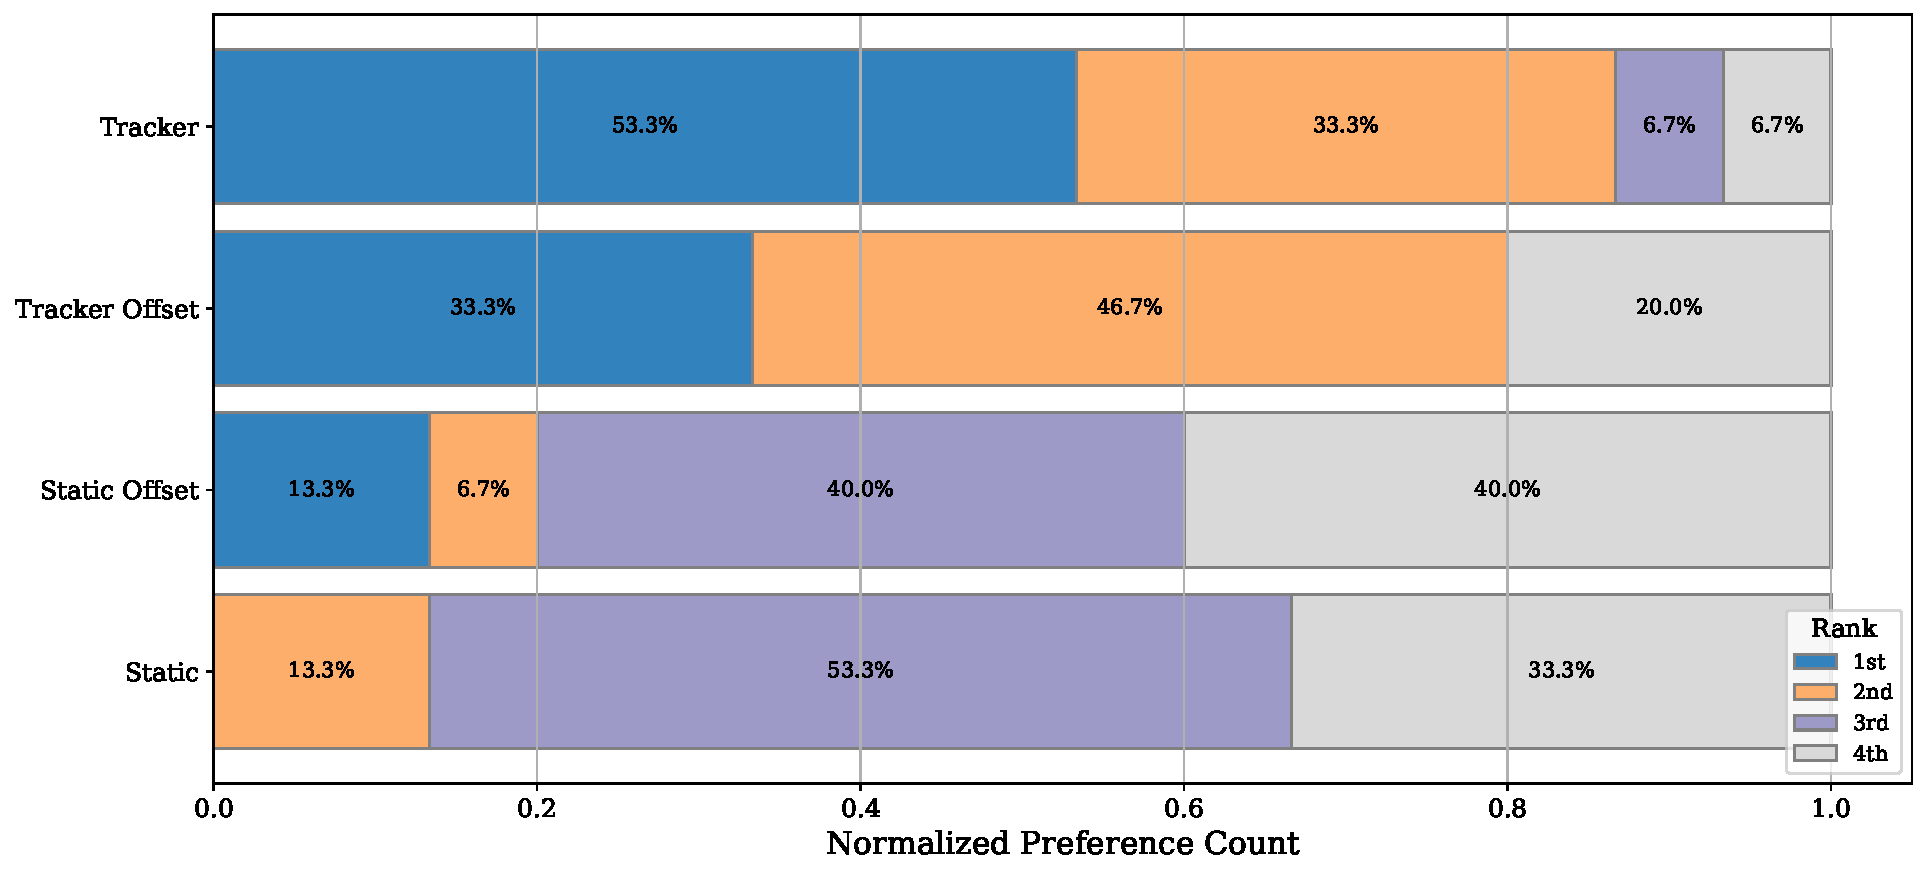
\includegraphics[width = 1.0\linewidth]{./evaluation/figures/survery/preferences.pdf}
\end{figureBox}

An overwhelming 87\% of participants chose either the TRACKER or TRACKER OFFSET condition as their top preference, indicating a strong preference for conditions that involved tracking. Interestingly, no participants ranked the STATIC condition as their first preference, despite it not being significantly slower than the TRACKER OFFSET condition according to the timing data we recorded. \\

We hypothesize that the strong bias against the STATIC and STATIC OFFSET condition may be due to the perceived naturalness and familiarity of the tracking conditions. Participants may have found these conditions more intuitive, possibly because they provided more visual information, even though this did not necessarily translate into improved task performance. \\

To analyze the preference rankings statistically, we performed a Friedman test. The results, presented in Table~\ref{tab:friedman-test}, show a significant difference in the rankings of the conditions, with a p-value of 0.00162. \\

\begin{table}[h!]
	\stepcounter{globalFigureCounter}
    \centering
    \caption{Friedman Test Results for Condition Preferences (Fig~\ref{fig:condition-preferences})}
    \label{tab:friedman-test}
    \begin{tabular}{lS[table-format=2.4]S[table-format=1.6]}
        \toprule
        \textbf{Statistic} & \textbf{Value} & \textbf{p-value} \\
        \midrule
        \texttt{Friedman Test Statistic} &  15.240 & 0.00162 \\
        \bottomrule
    \end{tabular}
\end{table}

These findings underscore the participants' preference for conditions that simulate a more dynamic and interactive experience, which they may have found more engaging or easier to understand.

\subsubsection{Further Analysis}
To avoid cluttering this section, graphs displaying the results of our study at a finer granularity can be found in the Appendix~\ref{app:results}. \\

\subsection{Discussion}

The results of our study provide valuable insights into the impact of display and interaction modalities on task performance and user preference in volumetric environments.

\subsubsection{Hypothesis Testing}
\begin{itemize}
	\item \textbf{H1}: There is a significant difference in task performance between 3D (TRACKER mode) and 2D (STATIC mode) interactions. Participants completed tasks faster and with higher precision in the 3D TRACKER condition when the display was directly in front of them, suggesting that 3D views enhance spatial understanding due to better depth cues like motion parallax. The advantage of 3D views diminishes with an offset.\\
	\item \textbf{H2}: Task performance varies significantly between direct hand interaction and tele-operation but only when the view was in 3D. Direct hand interaction in the 3D TRACKER condition resulted in superior performance, highlighting the effectiveness of natural hand movements in spatial tasks. The OFFSET conditions introduced challenges, suggesting that indirect manipulation impacts task accuracy.
\end{itemize}

\subsubsection{Precision and Task Complexity}
OFFSET conditions significantly hindered precision, suggesting that reduced motion parallax makes it difficult to judge distances. The STATIC condition's poorer performance, indicates challenges with depth perception and segment orientation in 2D views. 

\subsubsection{User Preferences}
There is a strong preference for TRACKER (3D) conditions, highlighting the subjective value of intuitive and interactive interfaces. The significant difference in rankings, as shown by the Friedman test, emphasizes the importance of user experience in technology adoption.

\subsubsection{Implications for Future Research and Design}
Future research should explore more variations of offset conditions and task complexities. In particular the impact of offsetting the interaction zone rather than the display should be investigated.  \\

Designers of Volumetric Display applications and experiences should prioritize direct hand interaction to enhance user experience and task performance. This is a difficulty for volumetric displays as almost always permeable/tangible so this not always achievable. \\